\documentclass{beamer}
\usepackage[size=a4]{beamerposter}
 
\usepackage{tikz}
\usetikzlibrary{arrows,automata,fit}

\begin{document}

\begin{frame}

\frametitle{Latent dirichlet allocation for classification}
~\\
\textbf{\large{Introduction to document analysis}}~\\
~\\
\begin{itemize}
\item \textbf{Term Frequency-Inverse Document Frequency (tf-idf),}~\\ \textit{Salton and McGill, 1983}~\\
$\rightarrow$ Reduces the arbitrary length documents to a fixed length of numbers~\\
~\\
\item \textbf{Latent semantici indexing}, \textit{Deerwester et al., 1990}~\\
$\rightarrow$ Similar to principal component analysis~\\
$\rightarrow$ Uses decomposition of the tf-idf matrix~\\
$ \rightarrow$ Preserving the most important semantic information~\\
~\\
\item \textbf{Probabilistic Laitent Semantic Indexing}, \textit{Hoffmann 1999}~\\
$\rightarrow$ Each word in a document is a sample from a mixture of multinomials~\\
$\rightarrow$The document is represented as a list of mixing proportions.~\\
$\rightarrow$ Limits : no generative model + complexity proportionnal to the size of the corpus
\end{itemize}

\end{frame}

\begin{frame}
\frametitle{Presentation of the LDA model}
%\section*{Presentation of the LDA model}
\begin{figure}i
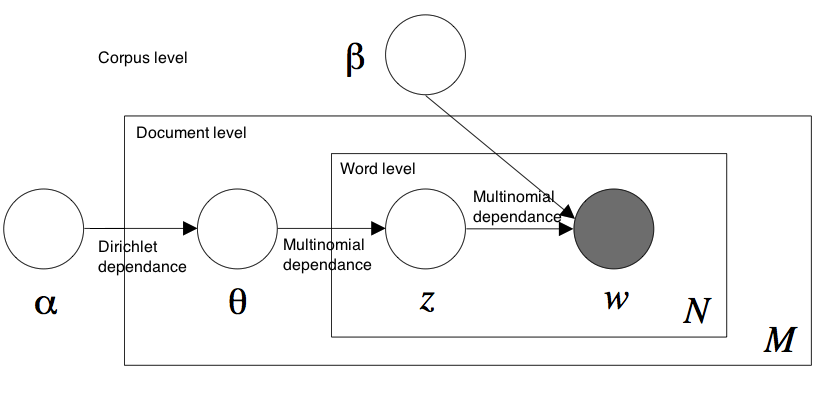
\includegraphics[width=18cm]{LDA}~\\
\end{figure}

$\rightarrow$Different model scales : corpus, document, word.~\\
~\\
$\rightarrow$Main assumption of the model : exchangeability of the documents and words in the document [De Finetti's theorem for the form of distribution]~\\
~\\
$\rightarrow$Procedure for document generation with respect to the graphical model~\\

\end{frame}

\begin{frame}
\frametitle{Presentation of the LDA model}
\begin{figure}
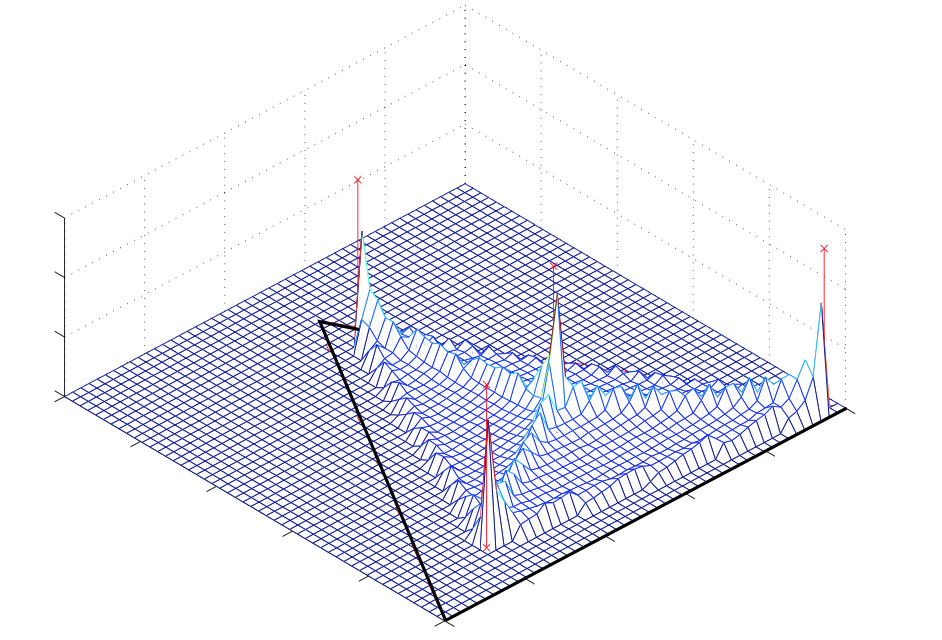
\includegraphics[width=12cm]{Simplex}~\\
\caption{Exemple with $ \theta \in $ 2D simplex }
\end{figure}
%\section*{Presentation of the LDA model}
$\rightarrow$ $\theta$ generates a multinomial topic distribution~\\
~\\
$\rightarrow$ This topic distribution generates words. In the case of 3 words, deterministic distribution on the vertices, midpoint of an edge gives probability 0.5 to two of the words, centroid of the triangle is the uniform distribution over the words~\\
~\\
$\rightarrow$Aim : estimation of corpus parameters $\alpha$ and $\beta$ for agenerative model of $p(\theta,z | \omega, \alpha, \beta)$

\end{frame}
\begin{figure}
	\centering
	\begin{tikzpicture}[->,>=stealth',shorten >=1pt,auto,node distance=5cm,
		semithick]
		\tikzstyle{every state}=[fill=white,draw=black,text=black]
		\node[state]         (A)                    {$\gamma$};
		\node [state]        (B) [below of=A]       {$\theta$};
		\node[state]         (C) [right of=A]       {$\phi$};
		\node[state]         (D) [below of=C]       {$z$};
		\node (B1) [draw=red, fit= (A) (B) (C) (D), inner sep=4cm] {};
		\node (B2) [draw=red, fit= (D) (C), inner sep=2cm] {};
		\node [yshift=3.0ex, black] at (B1.south) {$M$};
		\node [yshift=3.0ex, black] at (B2.south) {$N$};
		\path (A) edge              (B)
	              (C) edge              (D);
	\end{tikzpicture}
	\caption{Graphical model used to calculate the lower bound of the log-likelyhood for the LDA graphical model}
	\label{low_bound_model}
\end{figure}

\begin{frame}{Inference}
		\begin{itemize}
			\setlength{\itemsep}{100pt}
			\item Simplification of the model (Variational inference)
			\item Minimize KL-divergence to find $\gamma$ and $\phi$
			\item $\phi_{ni} = \frac{1}{Z} \beta_{i w_n} exp\left( E[log(\theta_i | \gamma] \right)$
			\item $\gamma_i = \alpha_i + \sum_{n=1}^{N} \phi_{ni}$
		\end{itemize}
\end{frame}


\begin{frame}{Parameter estimation}
		\begin{itemize}
			\setlength{\itemsep}{80pt}
			\item Compute a lower bound using variational model 
			\item Follow EM scheme
			\item E-step is the previous inference  
			\item M-step computes $\alpha$ and $\beta$:
				\begin{itemize}
					\item $\alpha$ computed using a Newton-Raphson scheme
					\item $\beta_{ij} = \sum_{d=1}^{M} \sum_{n=1}^{N_d} \phi_{ni} w_{dn}^j$
				\end{itemize}
		\end{itemize}
\end{frame}


\begin{frame}
\begin{table}[ht]
\begin{tabular}{c|c|c|c|c|c}
topic 1& topic 2& topic 3 & topic 4 & topic 5 & topic 6\\
\hline
Atheism     & Foundation  & Archive    & Article&Journalism&Plastic\\
Atheist     & Telephone   & Galactic   & Edu &Disappointing&Prometheus\\
Religion    & Evolution   & Files      & Wolkswagon &Elysium&Citroen\\
Evolution   & Books       & Information& Autobahns &Madonna&Tractors\\
Chritians   & History     & Article    & Locomotive &Game&Wolkswagen\\
Bible       & Planets & Writes     & Motorway &&Bicycling\\
Biblical    & Newsletter  & Selection  & Sportscar &&Competitive\\
Clerical    & National    & Create     & Municipalities &&Window\\
Church      & Science     & Integrated & Shaman &&Thread\\
Christianity& National    & Goto       & Schoolteacher &&Course\\
Christian   & Magazine    & Xgif       &&&\\
Catholic    & Scientific  & Header     &&&\\
Christ      & Complex     & Panel      &&&\\
Theism      & Random      & Algorithmic&&&\\
Believer    & Silicon     &	       &&&\\
	    & Space       &            &&&\\
	    & Dinosaurs   &            &&&\\
\end{tabular}
\end{table}
\end{frame}

\end{document}
